\section{Event storage} \label{section:security}
\large \textbf{Apache Kafka}\\
\normalsize
\textbf{Authentication mechanisms}\\
In a Kafka cluster, there are Kafka brokers and Zookeeper nodes. Only legitimate communication peers, namely, reliable Kafka clients, tools which also use Kafka clients internally such as Kafka Connect cluster for data integration and other Kafka brokers in the cluster can initiate connections to a Kafka broker. On the other hand, Zookeeper should be accessed only by Kafka brokers to maintain their metadata. Moreover, Kafka tools also expose REST endpoints for configuration and management such as deploying connectors in case of Kafka Connect. Kafka provides authentication mechanism to control access to all these endpoints \cite{kafkasecurity}.

In order to control access to a Kafka broker, Kafka supports two authentication mechanisms. The first is Transport Layer  Security/Secure Sockets Layer (TLS/SSL) protocol \cite{tls}. Users can configure each communication peer with a valid certificate signed by a mutual trusted Certification Authority (CA) and this will be used for 2-way authentication when establishing the connections between Kafka brokers or between a broker and a client. 

The second mechanism is Simple Authentication and  Security Layer (SASL) \cite{sasl}. Kafka supports 4 different SASL mechanisms out-of-the-box, namely, GSSAPI (Kerberos), PLAIN, SCRAM, and OAUTHBEARER. Users have the flexibility to choose the mechanism which fits to the security system in their existing infrastructures. A broker can also be configured to use multiple authentication mechanisms to support different groups of clients. 

With the Zookeeper soon to be removed from Kafka \cite{kafkaremovezookeeper}, the connection to Zookeeper will also become irrelevant. Nevertheless, in the current release 2.6.0, the connection to Zookeeper must still be protected by either TLS/SSL or SASL. For authentication with SASL, Zookeeper supports two mechanisms: Kerberos and DIGEST-MD5 \cite{zookeepersecurity}. However, the DIGEST-MD5 mechanism is already obsolete and should not be used in production.

Regarding the REST endpoints of the Kafka tools, Kafka supports authentication of connected users with TLS/SSL certificates. 

\textbf{Authorization mechanisms}\\
Kafka allows users to control different level of privilege and a different set of allowed operations for each connected client by providing an Access Control List (ACL) authorizer \cite{kafkasecurity}. This authorizer utilizes the identity of communication peers obtained from the authentication process to determine their access rights. The authorizer supports fine-grained access control for each client with each type of operation on each different resource. Users can define the access right for clients with the general format: \emph{Principal P is [Allowed/Denied] Operation O From Host H on any Resource R matching ResourcePattern RP}. In the current release, the access rights list is persisted by Kafka on Zookeeper. 

However, with the ACL authorizer, users must specify access rights for each and every client individually. Higher level of control, namely, Role-Based Access Control (RBAC) which allows to group multiple clients into one role adhered to only one access rule, is not possible. If this is needed, users must plug in a self-implemented authorizer which can bind the identities to different roles and define different access rules. 

On the other hand, for the connections from Kafka brokers to Zookeeper, Kafka automatically applies the access rules which allow only authenticated brokers to modify metadata stored on Zookeeper. This helps prevent unauthorized modification of metadata which may lead to cluster disruption.

\textbf{Encryption}\\
Kafka only supports encryption when transferring data using TLS/SSL \cite{kafkasecurity}. More specifically, the connections between Kafka brokers and clients, between two brokers, from broker to Zookeeper, and connections to REST endpoints of Kafka tools can be encrypted using the Public-Key Cryptography. Other than that, Kafka supports neither encryption of data at rest nor end-to-end encryption between two end clients.  

\begin{figure}[h]
	\centering
	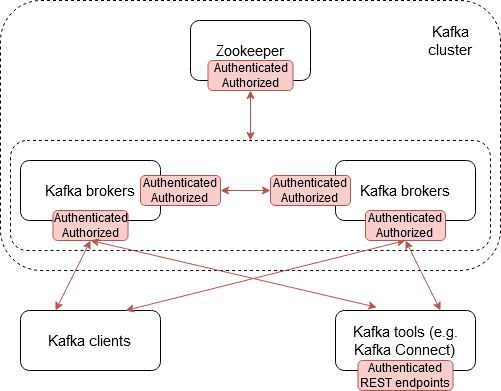
\includegraphics[width=10cm,height=7.5cm]{images/security-kafka.png}
	\caption{Secured Kafka cluster. Red links are encrypted.}
	\label{fig:securitykafka}
\end{figure}

\large \textbf{Apache Pulsar}\\
\normalsize
\textbf{Authentication mechanisms}\\
A Pulsar cluster comprises of multiple components. There are the Pulsar brokers, the Bookkeeper cluster and the Zookeeper nodes. In addition, when Pulsar Function or Pulsar IO is used and configured to be run separately from the brokers, there are also nodes of function workers in the cluster. All these components are interconnected. Pulsar provides different authentication mechanisms to protect these components against unauthorized accesses \cite{pulsarsecurity}.

For the Pulsar brokers and function worker nodes, Pulsar supports different authentication mechanisms. Clients connecting to a broker can be verified using mutual authentication of TLS/SSL protocol \cite{tls}. SASL authentication \cite{sasl} can also be used. Pulsar currently supports two SASL mechanisms which are OAUTHBEARER and GSSAPI (Kerberos). Moreover, with the OAUTHBEARER mechanism, Pulsar also provides a built-in tool to generate and verify token for client identification without having to rely on an additional authorization server. Authentication on Pulsar can also be done with Athenz, which is an open-source platform developed by Yahoo for authentication and authorization based on certificates

A Pulsar broker can be configured with multiple authentications mechanisms. Any client which wants to connect to this broker such as Pulsar producer, consumer, admin client, another broker or function worker must provide its identity with one of the supported authentication schemes of the broker. 

For the connections from Pulsar brokers to Zookeeper and Bookkeeper nodes, they can be protected with either SASL Kerberos authentication mechanism or TLS/SSL certificate-based authentication. Finally, for the connection from Bookkeeper to Zookeeper, users can also configure the authentication using TLS/SSL to control access.

\textbf{Authorization mechanisms}\\
To control access of authenticated clients to resources on Pulsar brokers and function workers, Pulsar provides a built-in authorizer to define ACL \cite{pulsarsecurity}.

The resources provided by Pulsar brokers are hierarchical. At the lowest level is topic from which clients can produce and consume messages. The next level is namespace which is a group of related topics. Then there is tenant resource which is a administrative unit consisting of multiple namespaces. Finally, at the highest level is the cluster. User can grant access to different type of resources on different levels for each authenticated client.

Pulsar does not support RBAC. Currently, there is not any mechanism to define and bind roles to clients and control access based on that.

For resources on Zookeeper and Bookkeeper, it is not documented. Therefore, it can be assumed that Pulsar manages the authorization internally and does not expose the control to users. 

\textbf{Encryption}\\
All connections in a Pulsar cluster can be encrypted with the TLS/SSL protocol. Moreover, Pulsar clients also supports end-to-end encryption \cite{pulsarsecurity}. This is achieved by combining symmetrical encryption and public-key encryption methods. A Pulsar producer can dynamically generate a symmetric key to encrypt payloads of messages. This symmetric key is then encrypted using a different public key in a public-private key pair and included in the header of the messages. On the consumer side, the consumer can use the corresponding private key to decrypt and retrieve the symmetric key used for payload encryption and then use that to read the messages. However, the distribution of the public-private key pair to the clients is not covered by Pulsar. Users must handle this task manually. 

\begin{figure}[h]
	\centering
	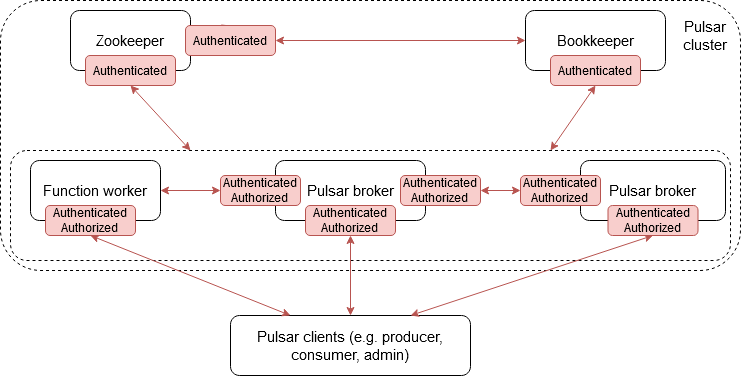
\includegraphics[width=15cm,height=6.5cm]{images/security-pulsar.png}
	\caption{Secured Pulsar cluster. Red links are encrypted.}
	\label{fig:securitypulsar}
\end{figure} 

\large \textbf{NATS Streaming}\\
\normalsize
\textbf{Authentication mechanisms}\\
A NATS Streaming server comprises of a NATS Server and a separated streaming module to provide durability of messages on top of the volatile NATS messaging system. 

NATS Streaming relies on the authentication mechanisms of normal NATS Server to control incoming accesses from clients \cite{normalnatsconfig}. In addition, since the streaming module is also a NATS client internally, it must also use the provided authentication mechanisms to connect to the NATS Server and serve requests from clients. On the other hand, since the durable storage is pluggable, it is beyond the scope of NATS Streaming to provide authentication for this component. Users must utilize the mechanism provided by the selected datastore.

Clients connected to the NATS server can be identified with mutual authentication using TLS/SSL protocol. NATS also provides a number of built-in authentication mechanisms. Users can configure the server and clients with a shared secret which will be used for authentication when a connection is established. NATS also provides a NATS-exclusive authentication mechanism which is public-key based and called NKey. Upon receiving connection request from a client, the server randomly generates a random value and challenges the client to encrypt that with its private key. The server can then verify the response from client by using the public key of the clients. With this authentication mechanism, NATS provides its own tool to generate public-key pairs and verify their legitimacy during authentication.

Nevertheless, apart from the authentication with TLS/SSL, the other authentication mechanisms are only NATS-specific. This lack of support for pluggable and common authentication mechanisms limits the adaptability of NATS Streaming to infrastructures with existing authentication services. In these cases, the security of the NATS system must be configured separately which can cause extra works on administration and maintenance.

\textbf{Authorization mechanisms}\\
The underlying NATS server of the streaming server also provides authorization mechanism to control access of individual clients on the resources \cite{normalnatsconfig}. Nevertheless, this mechanism is not compatible with the NATS Streaming \cite{natsauthorization}. 

More particularly, all subscription requests from clients to streaming channels are internally directed to the streaming module via a single non-persistent NATS channel designated for streaming subscriptions. The authorization mechanisms of NATS can only either block all requests of a client to this internal channel or allow any request to go through. As a result, it is not possible to allow a streaming client to subscribe to only a selective set of channels. 

Therefore, authorization is currently not supported on NATS Streaming. 

\textbf{Encryption}\\
Connections from clients to the NATS streaming server and from streaming module to the NATS server can be encrypted with the TLS/SSL protocol \cite{normalnatsconfig}. The connection from streaming module to the datastore is not covered by NATS. If this connection needs to be encrypted, users must choose the appropriate encryption scheme which is supported by the selected datastore.

Moreover, NATS Streaming also supports encryption of data at rest. The server can be configured with an encryption key and that will be used by the streaming module to encrypt the payload of all messages before persisting them in the durable storage \cite{natstoreencryption}. However, more fine-grained encryption such as different encryption keys for messages from different clients is not possible on NATS Streaming.
\begin{figure}[h]
	\centering
	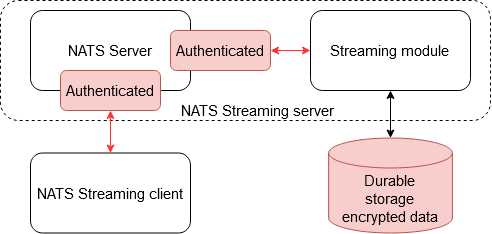
\includegraphics[width=10cm,height=6.5cm]{images/security-nats.png}
	\caption{Secured NATS Streaming cluster. Red links are encrypted.}
	\label{fig:securitynats}
\end{figure}
